\documentclass[11pt]{article}
\usepackage[latin1]{inputenc}
\usepackage{amsmath}
\usepackage{amsfonts}
\usepackage{amssymb}
\usepackage{graphicx}
\usepackage{setspace}
\usepackage[left=1.00in, right=1.00in, top=1.00in, bottom=1.00in]{geometry}
\usepackage[english]{babel}
\newcommand{\forceindent}{\leavevmode{\parindent=1.5em\indent}} % em = roughly width of uppercase ``M", or just over a third of a cm

\usepackage{fancyhdr}

\pagestyle{fancy}
\fancyhf{}
\rhead{University of Houston $|$ Political Science}
\lhead{Learning \LaTeX: Week 1} %% BE SURE TO CHANGE THIS EACH WEEK
\rfoot{Page \thepage}

\usepackage[round]{natbib}
\bibliographystyle{apsr}

\begin{document}
	
	\title{Learning \LaTeX \\
		\vspace{1cm}
	\large Week 1: Getting Started, Typesetting, and Basics \\
		\vspace{1cm}}
	\author{Philip D. Waggoner\footnote{{\texttt{philip.waggoner@gmail.com}}. This document was prepared by Philip Waggoner for the \textit{Weekly Workshops on Learning \LaTeX}, hosted by the Deparment of Political Science, University of Houston.}}
	\date{ } % getting rid of the automatic date
	\maketitle

\newpage

\tableofcontents

\newpage

\section{Introductory Remarks}
	
	\forceindent The popularity of \LaTeX\ is rapidly increasing, both in and out of political science. As such, to be prepared to engage with this increasingly popular and quite valuable tool, this workshop is designed to be a soft introduction to the program. Note that there are dozens of books, websites, and blogs dedicated to explaining and teaching \LaTeX. This is for two main reasons. First, like \texttt{R}, \LaTeX\ is open source, meaning any programmers can write packages and upload them to \texttt{CTAN} (The Comprehensive TeX Archival Network). Thus, the program is changing daily. Second, and most importantly, \LaTeX\ is very complex and can quickly get technical. While this workshop series will merely scratch the surface of everything the program can do, I highly recommend you take a look at some of these additional resources to help along the way. \\

	This is not to scare you, but rather motivate you to do two things. First, practice and apply everything we do here, at home on your own. Use \LaTeX\ everyday for everything you do. You will learn best and most quickly by forcing yourself to climb the steep learning curve. Once you do, you will likely be surprised by how quickly you pick it up. And second, Google any and all error messages and questions you have about whether the program can do something. As noted earlier, there are tons of sources to address problems, from the common to the technical. The best and most easily accessible resource is \texttt{https://tex.stackexchange.com/}. For those familiar, this is a lot like the stack exchange for \texttt{R} Also, this is an excellent resource for a variety of tutorials, issues, and problems: \texttt{https://www.sharelatex.com/}. \\

	In short, I hope this workshop will be useful and enjoyable. Please come ready to participate and ask questions. As I am not the final word on \LaTeX\ by any means, we will learn together. \\

	The workshops will meet most Fridays this semester at noon. We will meet anywhere from 1 -- 1.5 hours. The goal is to learn and retain for future use. Thus, too much information in a single session could limit the applicability of stuff we learn in this workshop. As such, it's important to reiterate that this workshop is intended to be a concise overview of \LaTeX\ and its basic features to set you up to be able to use it on your own down the line. But as such, this workshop series will merely scratch the surface. \\
	
	Finally, make sure to bring your own computers and come ready to participate. A lot of the class will be given to practicing that which we cover in the given workshop. There will inevitably be problems that arise, which we will do our best to address in the moment. \\

	Thus, in this first workshop, we will be covering the basics of opening and operating \LaTeX. By the end of the workshop, you should be able to understand and execute the following:

\begin{itemize}
	\item Opening the program
	\item Creating and typesetting a \LaTeX\ document
	\item Use footnotes
	\item Use basic punctuation, typeface, and commands
\end{itemize}

\newpage

\section{Getting Started}

	\forceindent Now that we are all set up, for the purposes of keeping everyone on the same page, we will be working primarily through \texttt{TeXStudio}. This is a lot like \texttt{R Studio}, where you can have easy shortcuts to commands, rather than having to type out each command. We will get to this in the next subsection below. \\

	It is important to note that \LaTeX\ is not a word processor, but is rather a formatter. This means you give it a series of commands, words included, and then you tell the file to print a document for you based on the commands you give it. And as many have said before, it bears repeating: computers are simultaneously brilliant and stupid; though they can do a ton, they are only as valuable as the information they are told to process. \LaTeX\ is no different, where it will only do what you tell it to do, and will not ``autocorrect", as millenials have become so accustomed to today. Thus, it is imperative to learn the mechanics of what's going on behind the scenes, to ensure proper formatting, resulting in a nice, pretty document. \\

	As such, there are \textbf{two} major things you need to know about the mechanics of how \LaTeX\ works. First, like \texttt{R}, most commands are possible through the use of a package. Packages are collections of commands that provide shortcuts to do stuff, on average (though some packages exist for specialized commands that are only possible with those commands). For example, the package ``threeparttable" is a good table creation package, which helps with things like putting footnotes on tables within the text. But you can also do this by inserting a simple textbox in a ``tabular" environment (more on this later). \\
	
	This brings us to the second key thing you need to understand about \LaTeX\, which is that the entire program functions through something called an ``environment." An environment is simply a space where you can type commands, beginning with the command ``begin", and ending with the command, ``end." And environments can and almost always are nested, where you work within a ``document" environment, to creatae a ``list" environment. While we will unpack these concepts over and over during this workshop, the key thing to remember is, to do virtually anything in \LaTeX\, you must be operating within an environment.

\newpage

\section{Simple Documents \& Typesetting}


	\forceindent Before we create a document, we need to learn, first how commands work, and then some basic commands to get us started. \\

	First, a command is how you ``call" something, or tell \LaTeX\ what you want it to do. The way we do any command is be preceding the substance of the command with the backslash. Then you follow it with whatever you want to do. \\

	Second, to see commands in practice, let's walk through starting a simple \LaTeX\ document by creating a document environment. Type...

\begin{figure}[!h]
	\includegraphics[scale=.6]{CODE} %[width=12cm, height=11cm] % to use instead of scale if need be
	%\centering
\end{figure}

	\forceindent To actually create the document, you need to typeset or ``compile" the document, which automatically generates a PDF, along with several other compilation files. For our purposes, you don't need to bother with these ancillary command logs and additional files, including error logs.\footnote{A quick word on errors: You will encounter many error messages in \LaTeX\ as you do and will in \texttt{R}. Though these are not nearly as useful in \LaTeX\ for helping you diagnose the problem, they are useful when they pop up in \texttt{TeXStudio}, in that they provide the line where the error is. When you click on some of the detailed information surrounding an error message, especially in bibliographies, which will be our second to last week, it will actually take you to the entry to help locate the problem. Beyond this, though, when you encounter an error message, simply go to the line it says, and figure out your mistake on your own. If you can't, Google the error message and likely something will come up for it.} Thus, in \texttt{TeXStudio}, click (or in TeXShop, you would click the big button aptly called, ``Typeset"),
	
\begin{figure}[!h]
	
\includegraphics[scale=.6]{TYPESET} \\ %[width=12cm, height=11cm] % to use instead of scale if need be
	%\centering
\end{figure}

Then, the output looks like... \\

\begin{figure}[!h]
	\includegraphics[scale=.5]{OUT} \\ %[width=12cm, height=11cm] % to use instead of scale if need be
	%\centering
\end{figure}

\newpage 

	Let's complicate things a little bit by including a heading with some more identifying information, sections, subsections, and subsubsections. These are some valuable and simple commands to produce a clean, organized document or paper. Let's walk through the following code together. \\

\begin{figure}[!h]
	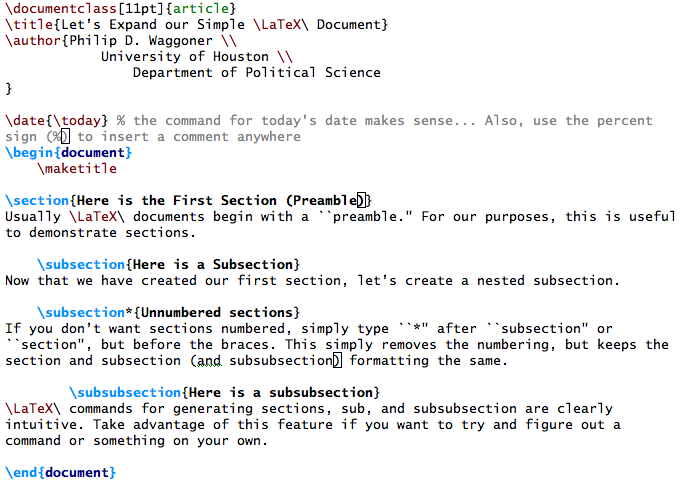
\includegraphics[scale=.6]{CODE2} \\ %[width=12cm, height=11cm] % to use instead of scale if need be
	%\centering
\end{figure}	

\newpage

Then, the output looks like... \\

\begin{figure}[!h]
	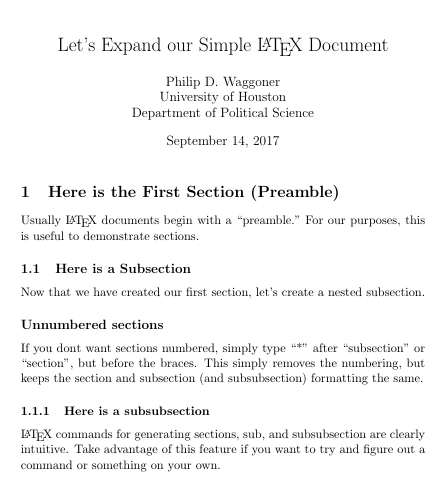
\includegraphics[scale=.7]{OUT2} \\ %[width=12cm, height=11cm] % to use instead of scale if need be
	\centering
\end{figure}

\newpage

\section{Footnotes}

	\forceindent We now know how to create a document in \LaTeX, as well as how to make it look a little bit nicer with sections and appropriate organization. Given that most of us will be using \LaTeX\ primarily for paper writing, at least in graduate school, the next extremely useful command is learning how to insert footnotes. Importantly, we could also use endnotes, but for two reasons I will pass on introducing this today. First, to use endnotes in \LaTeX, you need to install another package. Given the newness of the program at this point, let's keep things as simple as possible today. Second, footnotes are much more common in political science, and in general, much less frustrating when reading a paper. This is my humble opinion, but I don't enjoy flipping to the end of a paper to reference an endnote, when the information could just as easily be in front of me on the relevant page as a footnote. Therefore, let's stick with footnotes only today. \\

	You may be shocked to find out that the footnote command is... ``footnote." The only different from word processesors, that may take some getting used to, but that is actually much more intuitive, is the footnote is placed directly in the text of the processor, though in the typeset document it looks like a normal footnote that you would expect to see in a published paper. To get a better sense of precisely what I mean, let's first look at including a footnote in a block of text, and then we will look at the output. \\

	Start by including a footnote in our previous document with the sections. We will include the footnote in the beginning. Type... \\
	
\begin{figure}[!h]
	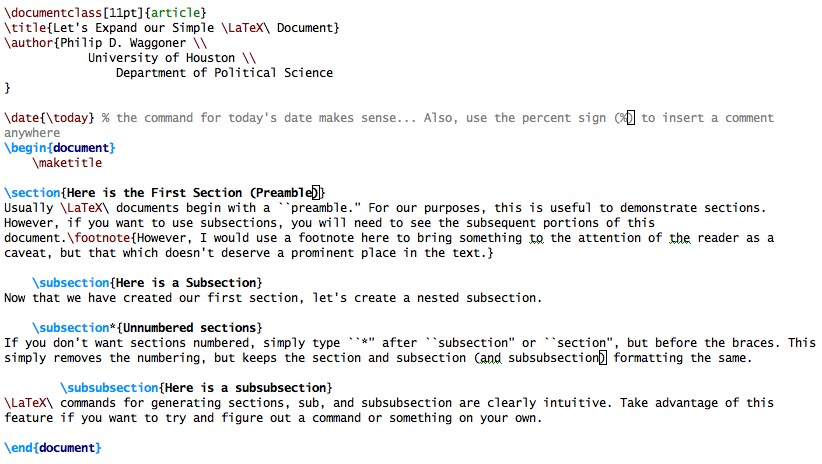
\includegraphics[scale=.7,, width=\textwidth]{CODE3} \\ %[width=12cm, height=11cm] % to use instead of scale if need be
	%\centering
\end{figure}

\newpage

Then, our output looks like...

\begin{figure}[!h]
	
\includegraphics[scale=.7]{OUT3} \\ %[width=12cm, height=11cm] % to use instead of scale if need be
	\centering
\end{figure}

\newpage

\section{Some Final Notes on Fonts and Other Commands}

	\forceindent Before looking at a few other commands, note that you can code the type face and font size, if you are unsatisfied with the default option when typesetting. To do so, the commands are also quite intuitive. \\

	For type face, here are the most common: \\

\begin{figure}[!h]
	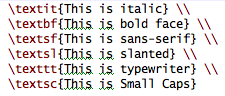
\includegraphics[scale=.7]{CODE4} \\ %[width=12cm, height=11cm] % to use instead of scale if need be
	%\centering
\end{figure}

	Then our output... \\

\begin{figure}[!h]
	
\includegraphics[scale=.7]{OUT4} \\ %[width=12cm, height=11cm] % to use instead of scale if need be
	\centering
\end{figure}	
	
	For font size, note the change can come from either lower or uppercase for the first letter of the command (e.g., ``large" versus ``Large.") Here are some examples: \\

\begin{figure}[!h]
	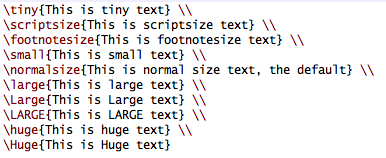
\includegraphics[scale=.7]{CODE5} \\ %[width=12cm, height=11cm] % to use instead of scale if need be
	%\centering
\end{figure}	

\newpage

	And our output... \\

\begin{figure}[!h]
	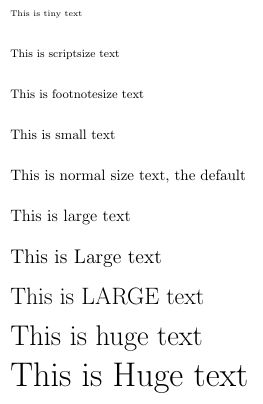
\includegraphics[scale=.7]{OUT5} \\ %[width=12cm, height=11cm] % to use instead of scale if need be
	\centering
\end{figure}

	To avoid overburdening you with too much information, yet out of a need to make you aware of the many other basic commands you will likely need to know, here is a great reource for a ton of commands: \texttt{https://www.ntg.nl/doc/biemesderfer/ltxcrib.pdf}.

\newpage

\section{Concluding Remarks}

	\forceindent We have seen a lot of new information today, and hopefully are starting to get the basic idea of \LaTeX. To review, we covered getting started, the basic idea of typesetting and creating documents in \LaTeX, some basic commands and ways to alter the font size and type face. I hope you feel a little less daunted by the program, and are excited to keep digging in. To reiterate, keep practicing this next week, and you will be much better off, both for next week's workshop, as well as in general in learning \LaTeX. 

\newpage

\section{Supplemental Resources \& Readings}

\vspace{1 cm}

\flushleft \textbf{A few websites (though there are many out there):}
\begin{enumerate}
	\item \texttt{https://tex.stackexchange.com/}
	\item \texttt{https://www.sharelatex.com/}
	\item \texttt{https://www.ntg.nl/doc/biemesderfer/ltxcrib.pdf}
	\item \texttt{https://www.latex-project.org/publications/}
	\item \texttt{http://www.math.harvard.edu/texman/}
	\item \texttt{https://tobi.oetiker.ch/lshort/lshort.pdf}
\end{enumerate}

\flushleft \textbf{And a few books:}
\begin{enumerate}
	\item Leslie Lamport. \LaTeX: A Document Preparation System. AddisonWesley,
	Reading, Massachusetts, second edition, 1994, ISBN 0-201-
	52983-1.
	
	\item Donald E. Knuth. The \TeX book, Volume A of Computers and Typesetting,
	Addison-Wesley, Reading, Massachusetts, second edition, 1984,
	ISBN 0-201-13448-9.
	
	\item Frank Mittelbach, Michel Goossens, Johannes Braams, David Carlisle,
	Chris Rowley. The \LaTeX\ Companion, (2nd Edition). Addison-Wesley,
	Reading, Massachusetts, 2004, ISBN 0-201-36299-6.
	
	\item Michel Goossens, Sebastian Rahtz and Frank Mittelbach. The \LaTeX\
	Graphics Companion. Addison-Wesley, Reading, Massachusetts, 1997,
	ISBN 0-201-85469-4.
\end{enumerate}


\end{document}
